\def\difficulty{2}
\sujet{Image Enhancement}
\label{tutorial:image_enhancement}

\begin{note}The objective of this tutorial is to implement some image enhancement methods, based on intensity transformations or histogram modifications. It will make use of statistical notions like probability density functions or cumulative distribution functions.\end{note}

\begin{figure}[H]
\centering\caption{The different processes of this tutorial will be applied on these images.}%
\subfloat[Osteoblasts.]{\includegraphics[height=.22\textheight]{osteoblaste.JPG}}
\hfill
\subfloat[Phobos (ESA/DLR/FU Berlin, CC-By-SA).]{\includegraphics[height=.22\textheight]{phobos.jpg}}%
\vspace*{-10pt}%
\label{fig:image_enhancement:enonce:examples}%
\end{figure}

\vspace*{-0.8cm}

\section{Intensity transformations (LUT)}
Two transformations will be studied: the $\gamma$ correction and the contrast stretching. They enable the intensity dynamics of the gray tone image to be changed. These two operators are based on the following Look Up Tables (LUT):

{
	\makeatletter
	\renewcommand\fs@ruled{\def\@fs@cfont{\bfseries}\let\@fs@capt\floatc@ruled
		\def\@fs@pre{\hrule height.8pt depth0pt \kern2pt}%
		\def\@fs@post{\kern2pt\hrule\relax}%
		\def\@fs@mid{\vskip2pt}%
		\let\@fs@iftopcapt\iftrue}
	\makeatother
\begin{figure}[H]
\subfloat[$\gamma$ correction LUT.]{%\includegraphics[width=6.25cm]{gamma.jpg}
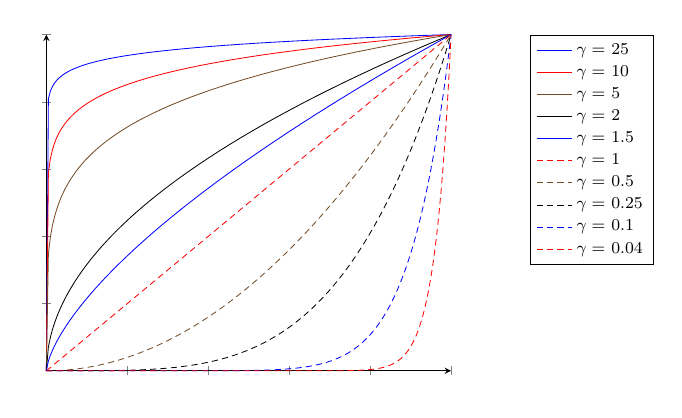
\begin{tikzpicture}[scale=0.75]
\begin{axis}[
  axis lines=middle,
  clip=false,
  ymin=0,
  xmin=0,
  xmax=1,
  ymax=1,
  xticklabels=\empty,
  yticklabels=\empty,
  legend style={at={(1.5,1)}},
  legend cell align=left
]
\newcounter{c}\setcounter{c}{1}

\pgfplotsinvokeforeach {25,10,5,2,1.5,1,0.5,0.25,0.1,0.04} {
  \addplot+[mark=none,samples=200,domain=0:1] {x^(1/#1)};
  %\node at (1-0.1*\thec, (1-.1*\thec)(1/#1)) {a};
  %\node[draw] at (.5,0.5) {\thec};
  \addlegendentry{\footnotesize $\gamma=$ #1};
  \stepcounter{c};
  }
\end{axis}
\end{tikzpicture}}\hfill
\subfloat[Contrast stretching LUT.]{
	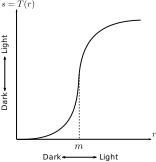
\includegraphics[width=.3\linewidth]{lut_stretching.pdf}
}
\end{figure}}

\begin{qbox}
\begin{enumerate}
	\item Test the transformation '$\gamma$ correction' on the image 'osteoblast'.
	\item Implement the operator 'contrast stretching' with the following LUT (also called cumulative distribution function $\mathrm{cdf}$), with $m$ being the mean gray value of the image, and $r$ being a given gray value:
	
	$$
	s=T(r)=\frac{1}{1+(m/r)^E}
	$$
	
	\item Test this transformation with different values of $E$ on the image 'osteoblast'.
\end{enumerate}
\end{qbox}

\begin{mcomment}
\begin{mremark}
You can have a look at \minline{imadjust} for $\gamma$ correction.
\end{mremark}
\end{mcomment}

\begin{pcomment}
\begin{premark}
The module \pinline{skimage.exposure} contains different methods for contrast enhancement, among them \pinline{adjust_gamma}.
\end{premark}
\end{pcomment}


\section{Histogram equalization}
\index{Histogram!Definition}
The objective is to transform the image so that its histogram would be constant (and its cumulative distribution function would be linear).
The notations are:
\begin{itemize}  \item $I$ is the image of $n$ pixels, with intensities between $0$ and $L$.
  \item $h$ is the histogram, defined by:
 \end{itemize}

$${\displaystyle h_I(k)=p(x=k)={\frac {n_{k}}{n}},\quad 0\leq k<L}$$

The following transformation $T(I)$ is called histogram equalization.\index{Histogram!Equalization}
$${\displaystyle T(x_k)=(L-1)\sum _{j=0}^{k}p(x_{j})} $$


 where $${\displaystyle \mathrm{cdf}_I(k)=\sum _{j=0}^{k}p(x_{j})} $$ is the cumulative distribution function (cumulative histogram). 

\begin{qbox}
\begin{enumerate}
	\item Compute and visualize the histogram of the image 'osteoblast'.
	\item Test this histogram equalization transformation on the image 'osteoblast' (with builtin functions) and visualize the resulting histogram.
	\item Code your own function.
	\item The corresponding LUT to this transformation is the cumulative sum of the normali\-zed his\-to\-gram. Evaluate and visualize this intensity transformation.
\end{enumerate}
\end{qbox}

\begin{mcomment}
\begin{mremark}
See the \minline{imhist}, \minline{histcounts} and \minline{histeq} functions.
\end{mremark}
\end{mcomment}

\begin{pcomment}
\begin{premark}
See the \pinline{numpy.histogram} and  \pinline{skimage.exposure} functions.
\end{premark}
\end{pcomment}

\section{Histogram matching}\index{Histogram!Matching}
The objective is to enhance the original image by matching its histogram with a modeled one. The principle is to transform the gray value $x_1$ of first image into $x_2$: $T(x_1)=x_2$ (see Fig.\ref{fig:enhancement:enonce:histmatching}). Based on the fact that $\mathrm{cdf}_1(x_1)=\mathrm{cdf}_2(x_2)$, the formula to find $x_2$ is: $$x_2=\mathrm{cdf}_2^{-1}\left(\mathrm{cdf}_1(x_1)\right).$$ 
As $x_1$ and $x_2$ are discrete values, this requires an interpolation.

\begin{figure}[htbp]
 \centering\caption{Histogram matching principle.}%
 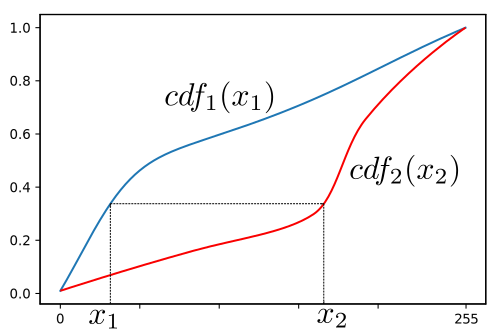
\includegraphics[width=.5\linewidth]{histmatching.pdf}%
 \label{fig:enhancement:enonce:histmatching}%
\end{figure}


\begin{qbox}
\begin{enumerate}
	\item Visualize the histogram of the image 'phobos'.
	\item Make the histogram equalization and visualize the resulting image.
	\item Construct a bi-modal histogram (for example) and code your own function for histogram matching.
\end{enumerate}
\end{qbox}

\begin{mcomment}
\begin{mremark}
See \minline{interp1} for interpolation and LUT application.
\end{mremark}
\end{mcomment}

\begin{pcomment}
\begin{premark}
See \pinline{numpy.interp} for interpolation and LUT application.
\end{premark}
\end{pcomment}
